\section{Introduction} % (fold)
\label{sec:introduction}

\HG is an interactive information visualization for people who want to get an overview of history. Our vision is to revolutionize how history is taught and learned. With our modern web technologies everyone is able to feel history in a nice, intuitive and simple way to understand the present and be prepared for the future.

\begin{figure}[H]
  \centering
  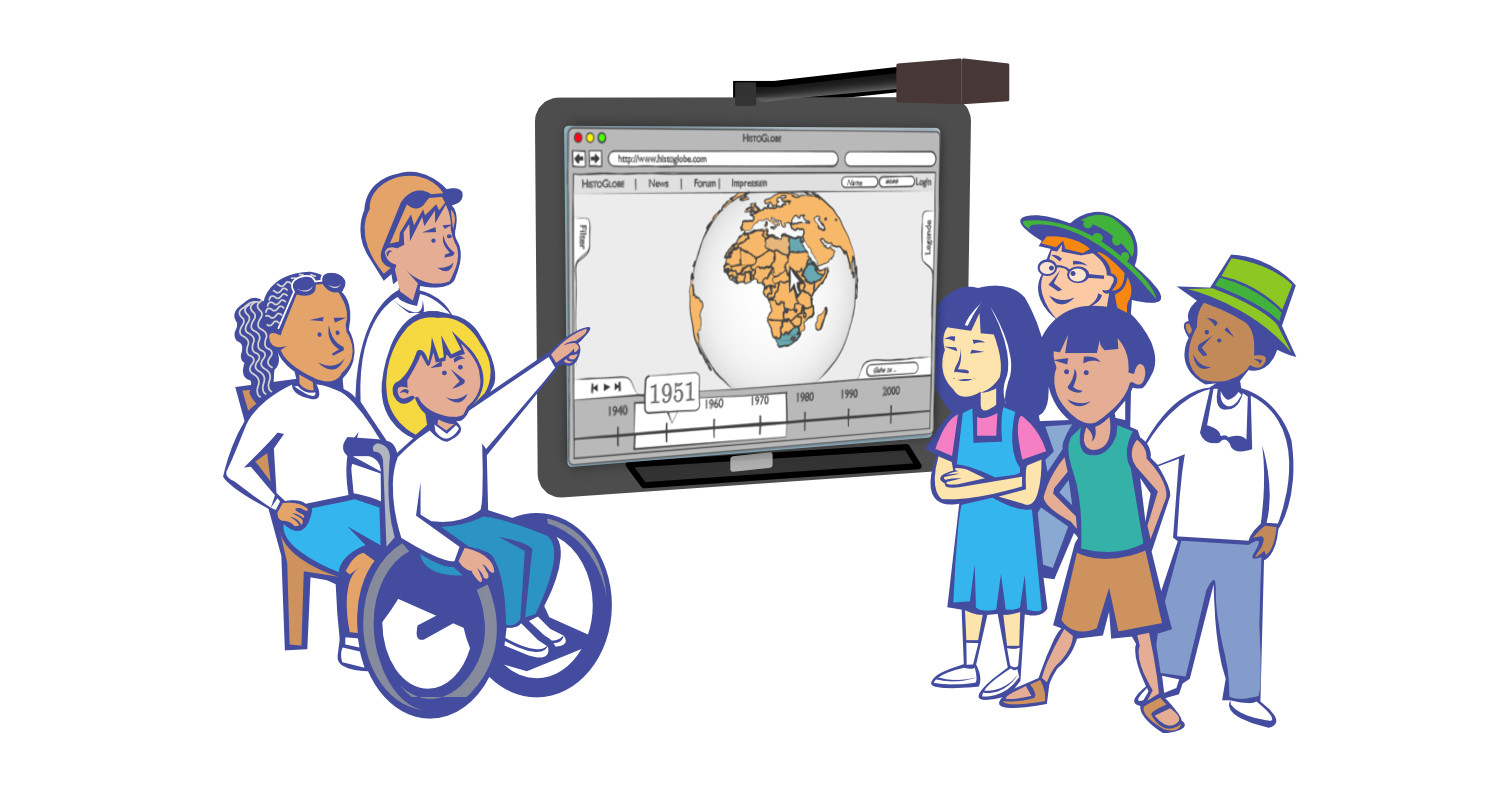
\includegraphics[width=0.8\textwidth]{graphics/everybody.jpg}
  \caption{Interactive Learning with \textsc{HistoGlobe}}
  \label{fig:everybody}
\end{figure}

Traditional media can not explain complicated relationships adequately: A book tells stories linearly, but history is complex and multi-dimensional. A static wall map can only display single frames of history, but hardly its dynamics.

We combined the geographical and temporal dimensions of history in one interface. The combination of time and space helps you to understand the historical context.

This way we are able to present students in school our way to experience history, guided by teachers or on their own.
\\
\\
This is \textsc{HistoGlobe}!

% section introduction (end)
